%!TEX program = lualatex
%\documentclass[aspectratio=169,compre%ss,9pt]{beamer}
\documentclass[compress,9pt,xcolor={dvipsnames,table}]{beamer}
\usepackage[T1]{fontenc}
%\usepackage{lmodern}
\usepackage{textcomp}
\usepackage{algorithm}
\usepackage{algorithmic}
\usepackage{tcolorbox}
\usepackage{fontspec}

\usepackage{polyglossia}
\setmainlanguage{english}
\usepackage{tabularx,ragged2e}
\usepackage{booktabs}
\usepackage{dtklogos}
\usepackage{arydshln}
\usepackage{chngpage}

\usepackage{multicol}
\usepackage[caption=false]{subfig}
\hypersetup{%
  colorlinks = true,
  linkcolor  = PineGreen!100!black
}

\usepackage{natbib}

\setbeamertemplate{itemize item}{\color{PineGreen}$\bullet$}
\setbeamertemplate{itemize subitem}{\color{PineGreen!25}$\circ$}
\setbeamercolor{enumerate item}{fg=PineGreen}

\setmainfont[]{Cardo} % sets the roman font
%\setsansfont[]{Alegreya} % sets the sans font % Vallkorn, Alegreya
\setsansfont[]{PT Sans} % sets the sans font
\setmonofont[]{Consolas} % sets the monospace font
\setbeamertemplate{navigation symbols}{}
    \expandafter\def\expandafter\insertshorttitle\expandafter{%
      \insertshorttitle\hfill%
      \insertframenumber\,/\,\inserttotalframenumber}

\usetheme{Szeged}
\usecolortheme{spruce}

\title[Smart usage of context information for the analysis, design and generation of power-aware polices for mobile sensing apps]{ Smart usage of context information for the analysis, design and generation of power-aware polices for mobile sensing apps}
\author[Rafael Perez Torres]{Presented by: Rafael Perez Torres\\[0.5cm] Thesis advisors:\\PhD Cesar Torres Huitzil\\PhD Hiram Galeana Zapien}
\institute{Cinvestav Tamaulipas}
%\date{\today}
\date{}

\begin{document}
\begin{frame}[plain]
  % {
  % \begin{center}
  % 
\includegraphics[scale=0.12]{../../../resources/images/vectors/cinvestav-logo-no-text}
  % \end{center}
  % }
  \begin{center}
  
\includegraphics[scale=0.12]{../../../resources/images/vectors/cinvestav-logo-no-text}
  \end{center}
  \titlepage
  
\end{frame}

%\frame{\maketitle}

\begin{frame}{Table of contents}
	\tableofcontents[hideallsubsections]
\end{frame}

\section{Introduction}
\subsection{Introduction}
\begin{frame}\frametitle{Introduction}
\begin{itemize}
	\item There is a massive adoption of mobile devices by society in almost any daily activity~\cite{Islam2014}.
	\begin{itemize}
		\item Any-where, any-time connectivity
		\item Possibility of installing new mobile applications
		\item Increasing computing, memory, and sensing capabilities
	\end{itemize}
	\item Sensing capabilities of smartphones improve interaction with user, turning mobile devices into \emph{omni-sensors} able to \emph{know} about their surrounding environment.
\end{itemize}
\end{frame}

\begin{frame}\frametitle{Introduction}
\begin{itemize}
	\item Hence, mobile devices have achieved a considerable degree of sensitivity that tries to mimic the sense of humans.
	\item In this way these devices have become \emph{context-aware}, which is translated to an increasing level of understanding about user's activity.
  \item \emph{Context} refers to a four-dimensional space composed of \emph{computing context}, \emph{physical context}, \emph{time context}, and \emph{user context}~\cite{Chen2000}.
\end{itemize}
\end{frame}


\begin{frame}\frametitle{Motivation}
\begin{itemize}
	\item Despite the increasing computing, storage and memory capabilities of smartphones, battery is not evolving at the same pace~\cite{Kjaergaard2012}.
	\item Each new generation of smartphones keeps improving and including new hardware embedded components, which imposes a higher energy demand.
	\item This limitation is highlighted when a continuous access to sensors data is needed, which is the core requirement of \textbf{mobile sensing applications}.
  \item Then it is mandatory for any mobile sensing application development to consider the energy constraint and implement mechanisms or strategies to optimize battery duration.
\end{itemize}
\end{frame}

\begin{frame}\frametitle{Motivation}

\begin{figure}[tb]
  \centering
  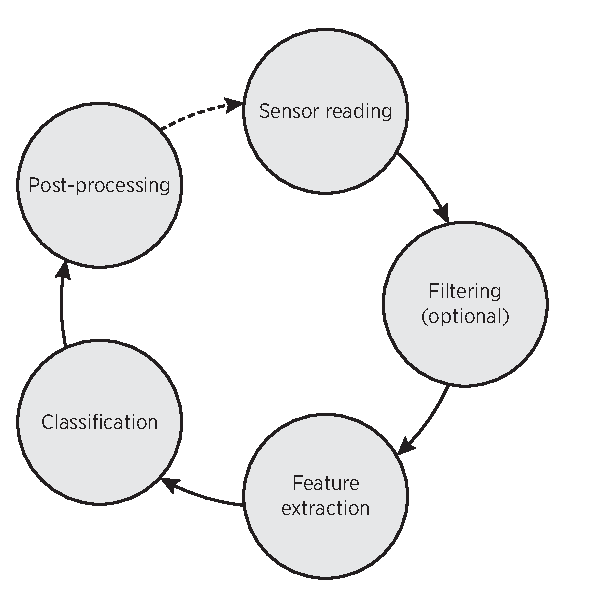
\includegraphics[width=\textwidth]{../../../resources/images/vectors/msa-stages}
  \caption{Stages of mobile sensing applications}
  \label{fig:msa-stages}
\end{figure}

\begin{itemize}
  \item There is a tradeoff between the accuracy of context information retrieved and the associated energy consumption~\cite{Sim2014,Rachuri2012}.
\end{itemize}
\end{frame}


\section{Hypothesis and problem statement}
\subsection{Hypothesis and problem statement}
\begin{frame}\frametitle{Hypothesis}
\begin{tcolorbox}[title=Hypothesis,colframe=PineGreen]
Intelligent policies produced through context information built from sensors data can be employed to reduce the energy consumption in a mobile device when performing continuous sensor readings.
\end{tcolorbox}

{
\small
\begin{itemize}
	\item An intelligent policy is a special rule that defines how sensors should be accessed in order to reduce the energy consumption and achieve the requirements of a mobile app.
	It is intelligent in terms of self-adaptness to changes detected in context information.
	\item This research work aims to employ data coming from GPS and inertial sensors (accelerometer) in order to obtain context information about user mobility that helps to adapt the usage of sensors and reduce energy consumption.
\end{itemize}
}
\end{frame}


\begin{frame}\frametitle{Problem statement}
\begin{tcolorbox}[title=Problem statement: Mobility pattern identification,colframe=PineGreen]
\small
Given a set $V = \left\{v_{1}, v_{2}, \dotsc, v_{n}\right\}$ of data values read from sensor $S$ in the time interval $T  \in [t_{1}, t_{2}]$, identify the current mobility pattern $p_{S}$ that represents the activity of user.

\begin{equation}
  \text{PatternIdentifier}( V ) \longrightarrow{} p_{S} \in Patterns
\end{equation}

Where $Patterns$ is a set of patterns that represent an interesting state in user mobility, specifically the set $\left\{no\_movement, walking, running, vehicle\_transportation\right\}$.
\end{tcolorbox}
\end{frame}

\begin{frame}\frametitle{Problem statement}
\begin{tcolorbox}[title=Problem statement: Policy generation,colframe=PineGreen]
\small
Given the set of detected mobility patterns $\mathcal{P} = \{ p_{S_1}, p_{S_2}, \ldots, p_{S_n} \}$ in data from sensors $\mathcal{S} = \{ S_1,S_2,\ldots, S_n \}$, parameters for assigning weight to energy $e$ and accuracy $a$, and physical constraints status $c$ of a mobile device, find a policy that select the proper set of sensors $\mathcal{S}_{new}$ and its associated configuration $\mathcal{S}_{new_{conf}}$  while meeting application requirements.

\begin{equation}
  \text{PolicyGeneration}( \mathcal{P}_{\mathcal{S}}, e, a, c ) \longrightarrow{} \mathcal{S}_{new}, \mathcal{S}_{new_{conf}}
\end{equation}

The $\mathcal{S}_{new_{conf}}$ configuration is referred as the \emph{duty cycle} of associated sensor.
\end{tcolorbox}
\end{frame}

\section{Objectives}
\subsection{Objectives}
\begin{frame}\frametitle{Objectives}
\begin{tcolorbox}[title=Main objective,colframe=PineGreen]
To reduce energy consumption in the mobile sensing apps, which perform continuous sensor readings, through power-aware policies generated from context information obtained from sensors data.
\end{tcolorbox}
\end{frame}

\begin{frame}\frametitle{Objectives}
\begin{tcolorbox}[title=Particular objectives,colframe=PineGreen]
\small
\begin{itemize}
  \item To identify mobility patterns from context information obtained from an inertial sensor (accelerometer) and location providers (GPS, WPS).
  \item To generate policies for a smart sensors' usage from identified mobility patterns, accuracy and energy requirements of mobile application, and status of mobile device's constraints. 
  \item To ease the development of mobile sensing applications that require user location tracking, i.e., LBS, by means of a middleware that isolates the complexity of sensors' access and the associated efficient energy management.
\end{itemize}
\end{tcolorbox}
\end{frame}


\section{Methodology}
\subsection{Methodology}
\begin{frame}\frametitle{Methodology}
\begin{enumerate}
  \item Research on the characteristics of data delivered by sensors, (GPS and accelerometer).
  \item Definition and selection of mobility patterns to be identified.
  \item Research and selection of algorithms to detect mobility patterns of user based on data delivered by GPS and accelerometer.
  \item Creation of the pattern identifier element (PIE).
  \item Creation of the policy generator element (PGE).
  \item Development of a software element (SE) that integrates both PIE and PGE.
  \item Experimentation.
\end{enumerate}
\end{frame}


\section{Schedule}
\subsection{Schedule}
\begin{frame}{Schedule}
  \definecolor{colorA}{gray}{0.85}
  \definecolor{colorB}{gray}{0.95}
  \definecolor{colorStep}{gray}{1}

  \newlength{\longitudCelda}
  \setlength{\longitudCelda}{75mm}

  \begin{table}[!h]
  {
    \scalebox{0.63}{
    %\scalebox{0.6}{
    \small
      \begin{tabular*}{16.5cm}{lp{\longitudCelda}*{12}{c}}
          & & \multicolumn{3}{ c: }{\tiny SEP '14 - AUG '15}  & \multicolumn{3}{ c: }{\tiny SEP '15 - AUG '16} & \multicolumn{3}{ c: }{\tiny SEP '16 - AUG '17} & \multicolumn{3}{ c }{\tiny SEP '17 - AUG '18} \\
          \cline{3-14}

          \multicolumn{2}{c:}{}
          & \tiny 1\textsuperscript{st} & \tiny 2\textsuperscript{nd} & \multicolumn{1}{c:}{ \tiny 3\textsuperscript{rd}}
          & \tiny 1\textsuperscript{st} & \tiny 2\textsuperscript{nd} & \multicolumn{1}{c:}{ \tiny 3\textsuperscript{rd}}
          & \tiny 1\textsuperscript{st} & \tiny 2\textsuperscript{nd} & \multicolumn{1}{c:}{ \tiny 3\textsuperscript{rd}}
          & \tiny 1\textsuperscript{st} & \tiny 2\textsuperscript{nd} &  \tiny 3\textsuperscript{rd} \\
          \cline{3-14}

          \rowcolor{colorStep}
          & \multicolumn{1}{c}{\scriptsize \textsc{Step I}}  & & & & & & & & & & & & \\
          % First year
          \rowcolor{colorA}
          1 & \multicolumn{1}{p{\longitudCelda}:}{Research on characteristics of data delivered by GPS receiver} &
          \cellcolor[gray]{0.3} & & &
          & & &
          & & &
          & & \\

          %\hdashline
          \rowcolor{colorStep}
          & \multicolumn{1}{c}{\scriptsize \textsc{Step II}}  & & & & & & & & & & & & \\

          \rowcolor{colorB}
          2 & \multicolumn{1}{p{\longitudCelda}:}{Coding a sample app to gather GPS data from smartphone} &
          \cellcolor[gray]{0.3} & & &
          & & &
          & & &
          & & \\

          \rowcolor{colorA}
          3 & \multicolumn{1}{p{\longitudCelda}:}{Analysis of data delivered by the mobile app} &
          \cellcolor[gray]{0.3} & & &
          & & &
          & & &
          & & \\

          \rowcolor{colorB}
          4 & \multicolumn{1}{p{\longitudCelda}:}{Selection of the mobility patterns} &
          \cellcolor[gray]{0.3} & \cellcolor[gray]{0.3} & &
          & & &
          & & &
          & & \\

          \rowcolor{colorA}
          5 & \multicolumn{1}{p{\longitudCelda}:}{Creation of the formal definition of mobility pattern} &
          & \cellcolor[gray]{0.3} & &
          & & &
          & & &
          & & \\

          %\hdashline
          \rowcolor{colorStep}
          & \multicolumn{1}{c}{\scriptsize \textsc{Step III}}  & & & & & & & & & & & & \\

          \rowcolor{colorB}
          6 & \multicolumn{1}{p{\longitudCelda}:}{Research on algorithms for pattern recognition from GPS data} &
          & \cellcolor[gray]{0.3} & &
          & & &
          & & &
          & & \\

          \rowcolor{colorA}
          7 & \multicolumn{1}{p{\longitudCelda}:}{Definition of metrics for evaluating algorithms} &
          & \cellcolor[gray]{0.3} & \cellcolor[gray]{0.3} &
          & & &
          & & &
          & & \\

          \rowcolor{colorB}
          8 & \multicolumn{1}{p{\longitudCelda}:}{Evaluation of algorithms} &
          & & \cellcolor[gray]{0.3} &
          & & &
          & & &
          & & \\

          \rowcolor{colorA}
          9 & \multicolumn{1}{p{\longitudCelda}:}{Selection of proper algorithm(s)} &
          & & \cellcolor[gray]{0.3} &
          & & &
          & & &
          & & \\

          % Second year
          \rowcolor{colorStep}
          & \multicolumn{1}{c}{\scriptsize \textsc{Step IV}}  & & & & & & & & & & & & \\

          \rowcolor{colorB}
          10 & \multicolumn{1}{p{\longitudCelda}:}{Definition \& representation of parameters accepted by PIE} &
          & & &
          \cellcolor[gray]{0.3} & & &
          & & &
          & & \\

          \rowcolor{colorA}
          11 & \multicolumn{1}{p{\longitudCelda}:}{Elaboration of the PIE} &
          & & &
          \cellcolor[gray]{0.3} & \cellcolor[gray]{0.3} & &
          & & &
          & & \\

          %\hdashline
          \rowcolor{colorStep}
          & \multicolumn{1}{c}{\scriptsize \textsc{Step V}}  & & & & & & & & & & & & \\

          \rowcolor{colorB}
          12 & \multicolumn{1}{p{\longitudCelda}:}{Definition \& representation of parameters accepted by PGE} &
          & & &
          & & \cellcolor[gray]{0.3} &
          & & &
          & & \\

          \rowcolor{colorA}
          13 & \multicolumn{1}{p{\longitudCelda}:}{Creation of the formal definition of policy} &
          & & &
          & & \cellcolor[gray]{0.3} &
          & & &
          & & \\

          \rowcolor{colorB}
          14 & \multicolumn{1}{p{\longitudCelda}:}{Elaboration of the PGE} &
          & & &
          & & \cellcolor[gray]{0.3} &
          \cellcolor[gray]{0.3} & \cellcolor[gray]{0.3} & &
          & & \\

          %\hdashline
          \rowcolor{colorStep}
          & \multicolumn{1}{c}{\scriptsize \textsc{Step VI}}  & & & & & & & & & & & & \\

          \rowcolor{colorA}
          15 & \multicolumn{1}{p{\longitudCelda}:}{Analysis of elements involved into software abstractions} &
          & & &
          & & &
          & \cellcolor[gray]{0.3} & &
          & & \\

          \rowcolor{colorB}
          16 & \multicolumn{1}{p{\longitudCelda}:}{Research on Android API for specialized components} &
          & & &
          & & &
          & \cellcolor[gray]{0.3} & &
          & & \\

          \rowcolor{colorA}
          17 & \multicolumn{1}{p{\longitudCelda}:}{Coding-development of the SE} &
          & & &
          & & &
          & \cellcolor[gray]{0.3} & \cellcolor[gray]{0.3} &
          & & \\

          %\hdashline
          \rowcolor{colorStep}
          & \multicolumn{1}{c}{\scriptsize \textsc{Step VII}}  & & & & & & & & & & & & \\

          % Fourth year
          \rowcolor{colorB}
          18 & \multicolumn{1}{p{\longitudCelda}:}{Definition of experiments} &
          & & &
          & & &
          & & \cellcolor[gray]{0.3} &
          & & \\

          \rowcolor{colorA}
          19 & \multicolumn{1}{p{\longitudCelda}:}{Development of mobile apps for running the experimentation} &
          & & &
          & & &
          & & \cellcolor[gray]{0.3} &
          & & \\

          \rowcolor{colorB}
          20 & \multicolumn{1}{p{\longitudCelda}:}{Execution of the experimentation} &
          & & &
          & & &
          & & \cellcolor[gray]{0.3} &
          \cellcolor[gray]{0.3} & & \\

          \rowcolor{colorA}
          21 & \multicolumn{1}{p{\longitudCelda}:}{Results analysis} &
          & & &
          & & &
          & & &
          \cellcolor[gray]{0.3} & & \\

          % Required tasks
          %\hdashline
          \rowcolor{colorStep}
          & \multicolumn{1}{c}{\scriptsize \textsc{Required tasks}}  & & & & & & & & & & & & \\

          \rowcolor{colorB}
          22 & \multicolumn{1}{p{\longitudCelda}:}{Related subject courses} &
          \cellcolor[gray]{0.3} & \cellcolor[gray]{0.3} & \cellcolor[gray]{0.3} &
          & & &
          & & &
          & & \\

          \rowcolor{colorA}
          23 & \multicolumn{1}{p{\longitudCelda}:}{Publication of results} &
          & & &
          & & &
          & & &
          \cellcolor[gray]{0.3} & \cellcolor[gray]{0.3} & \cellcolor[gray]{0.3} \\

          \rowcolor{colorB}
          24 & \multicolumn{1}{p{\longitudCelda}:}{Thesis writing} &
          & & &
          & & &
          & & &
          \cellcolor[gray]{0.3} & \cellcolor[gray]{0.3} & \cellcolor[gray]{0.3} \\

      \end{tabular*}
    }
  } % begin table
  %\caption{Schedule of activities (each column represents a four months period)}
  %\label{tbl-schedule}
  \end{table}
\end{frame}


\section{Contributions}
\subsection{Contributions}
\begin{frame}\frametitle{Contributions}
\begin{itemize}
  \item A mechanism for detecting mobility patterns from the data read by sensors of mobile devices (especifically GPS and accelerometer).
  \item A mechanism for generating policies for accessing sensors.
  %Besides the identified mobility pattern, such mechanism also considers mobile application's requirements (energy and accuracy hints), and the status of device constraints.
  The produced policies will allow to perform an intelligent usage of smartphone's sensing infrastructure in continuous sensor readings, reducing the energy consumption.
  \item A middleware implementing the previous mechanisms, easing the development of mobile sensing applications.
\end{itemize}
\end{frame}


\section{Developed work}
\subsection{Developed work}
\begin{frame}\frametitle{Brief state of art revision}
\begin{figure}[tb]
  \centering
  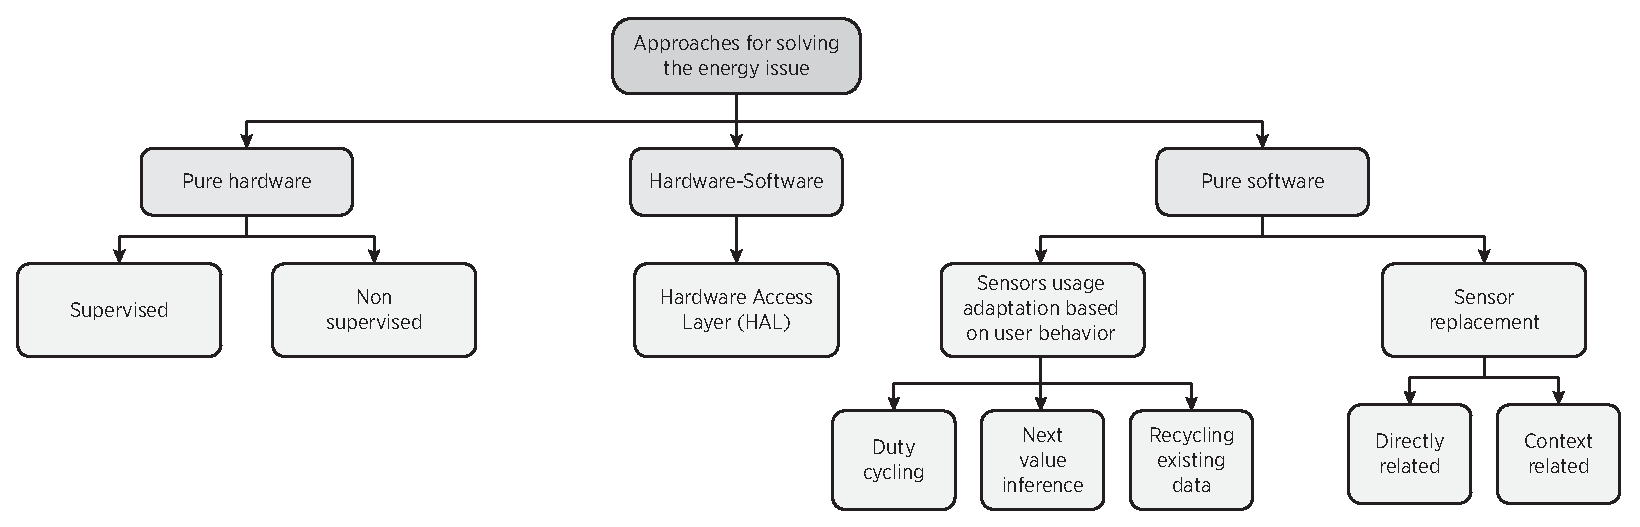
\includegraphics[width=\textwidth]{../../../resources/images/vectors/approaches-taxonomy}
  \caption{Taxonomy of solutions}
  \label{fig:taxonomy}
\end{figure}
\end{frame}

\begin{frame}\frametitle{Brief state of art revision}
\begin{figure}[tb]
  \centering
  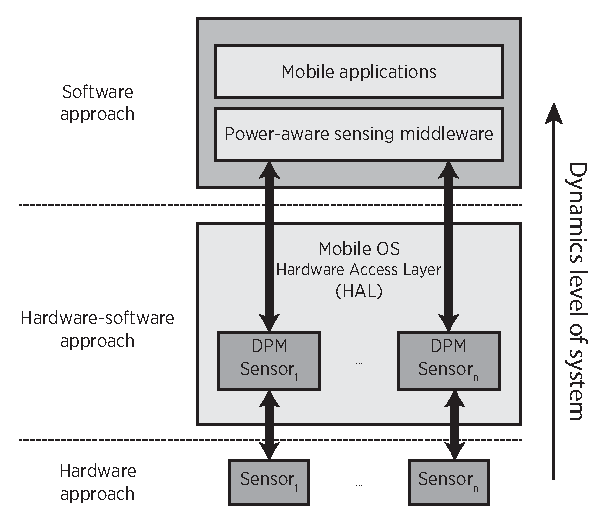
\includegraphics[scale=0.72]{../../../resources/images/vectors/approaches-distribution}
  \caption{Distribution of approaches across mobile platform's layers}
  \label{fig:distribution}
\end{figure}
\end{frame}

\begin{frame}\frametitle{Basic scenario}
\begin{figure}[tb]
  \centering
  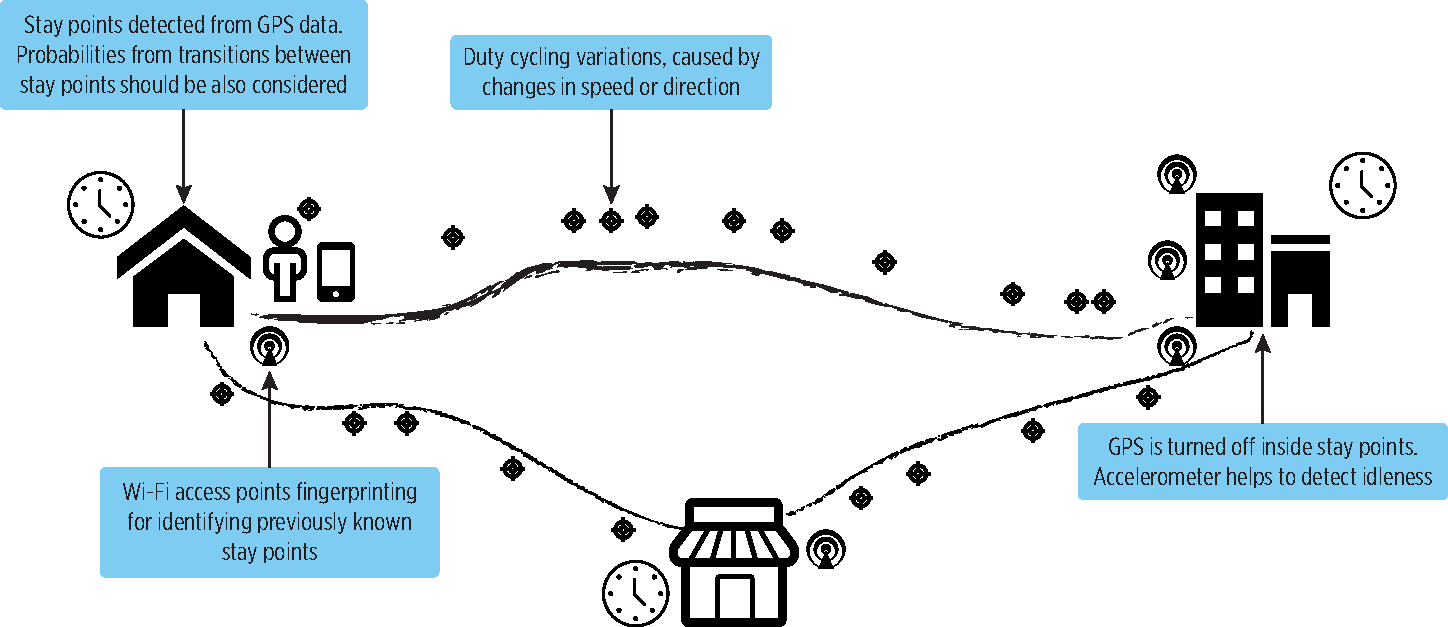
\includegraphics[width=\textwidth]{../../../resources/images/vectors/scenario}
  \caption{Basic scenario}
  \label{fig:scenario}
\end{figure}
\end{frame}

\begin{frame}\frametitle{Proposed solution}
\begin{figure}[tb]
  \centering
  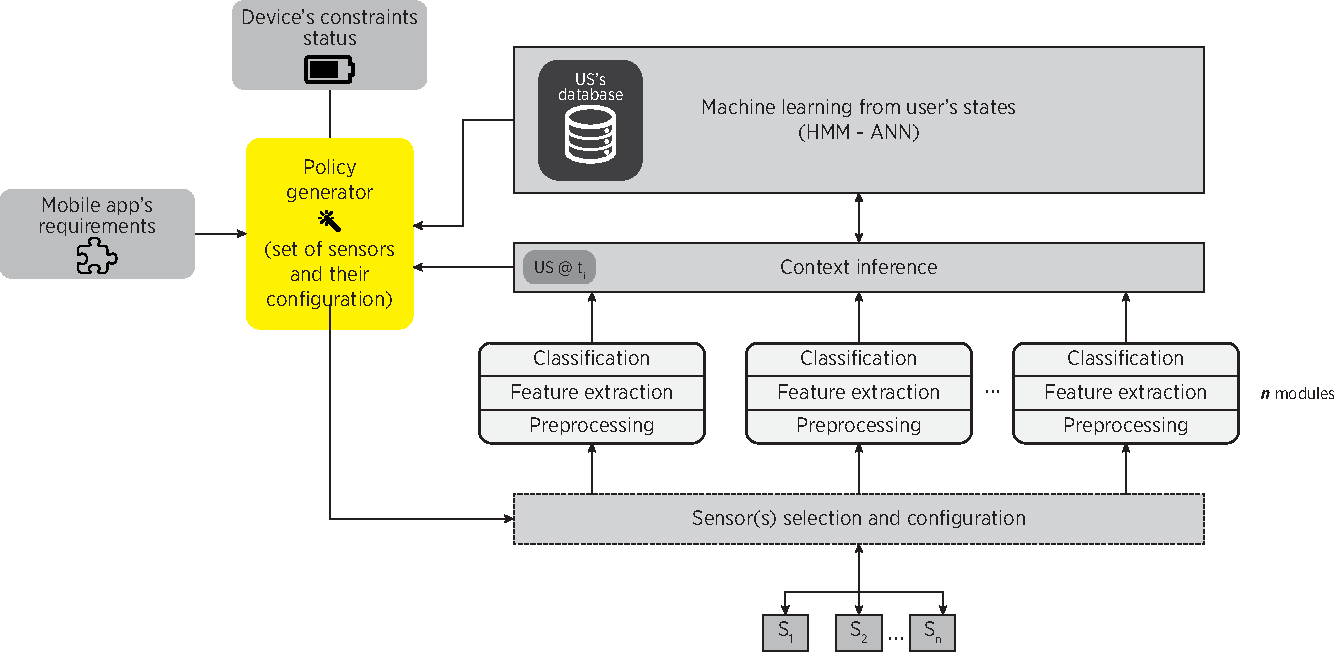
\includegraphics[width=\textwidth]{../../../resources/images/vectors/policy-manager-incorporation}
  \caption{Overview of current solution}
  \label{fig:solution}
\end{figure}
\end{frame}

\subsection{References}
\bibliographystyle{plain}
% \bibliographystyle{unsrtnat}
% \tiny
\bibliography{../../../resources/references/bibliography}

\end{document}
